% This template is created by SV Bùi Vân Anh, và Thầy Nguyễn Tiến Hòa từ phòng Lab xử lý tín hiệu băng gốc hệ thống 5G. Chúng tôi rất vui nếu được nhắc đến trong lời cảm ơn.
%%%%%%%%%%%%%%%%%%%%%%%%%%%%%%%%%%%%%%%%%%%%%%%%%%%%%%%
\documentclass{article} % Tạo một bản báo cáo
%\usepackage[utf8]{inputenc}
\usepackage[T5]{fontenc} % Để sử dụng Tiếng Việt
\usepackage[fontsize=13pt]{scrextend} % Set fontsize=13pt
%\usepackage[paperheight=29.7cm,paperwidth=21cm,right=2cm,left=3cm,top=2cm,bottom=2.5cm]{geometry}% Chuẩn A4, căn lề phải, trái, trên, dưới.
\usepackage[paperheight=29.7cm,paperwidth=21cm,right=2cm,left=3cm,top=2cm,bottom=2.5cm,twoside]{geometry}% Chuẩn A4, căn lề phải, trái, trên, dưới.
\usepackage{mathptmx} % Time New Roman
\usepackage{amsmath}
\usepackage{graphicx} % Thư viện chèn ảnh
\usepackage{float} % Set vị trí chèn ảnh
\usepackage{tikz} % Thư viện tạo khung bìa
\usetikzlibrary{calc} % Thư viện tikz
\usepackage{indentfirst} % Thư viện thụt đầu dòng
\usepackage{booktabs} % To thicken table lines
\renewcommand{\baselinestretch}{1.2} % Giãn dòng 1.2
\setlength{\parskip}{6pt} % Spacing after
\setlength{\parindent}{1cm} % Set khoảng cách thụt đầu dòng mỗi đoạn
\usepackage{titlesec} % Thư viện để set up các kiểu chữ
\setcounter{secnumdepth}{4} % 4 Heading
\titlespacing*{\section}{0pt}{0pt}{30pt} % Heading 1
% Định dạng hiển thị: Tự động thêm tiền tố "CHƯƠNG X. "
\titleformat{\section}{\fontsize{16pt}{0pt}\selectfont \bfseries \centering}{CHƯƠNG \thesection.\ }{0pt}{}

\titlespacing*{\subsection}{0pt}{10pt}{0pt} % Heading 2
\titleformat*{\subsection}{\fontsize{14pt}{0pt}\selectfont \bfseries}

\titlespacing*{\subsubsection}{0pt}{10pt}{0pt} % Heading 3
\titleformat*{\subsubsection}{\fontsize{13pt}{0pt}\selectfont \bfseries \itshape}

\titlespacing*{\paragraph}{0pt}{10pt}{0pt} % Heading 4
\titleformat*{\paragraph}{\fontsize{13pt}{0pt}\selectfont \itshape}

\renewcommand{\figurename}{\fontsize{12pt}{0pt}\selectfont \bfseries Hình}
\usepackage[font=bf]{caption}
\captionsetup[figure]{labelsep=space}

\renewcommand{\tablename}{\fontsize{12pt}{0pt}\selectfont \bfseries Bảng}
\captionsetup[table]{labelsep=space}

% Tự động đánh số theo dạng Section.Số và tự reset ở mỗi chương mới
\numberwithin{equation}{section}
\numberwithin{figure}{section}
\numberwithin{table}{section}

\usepackage{tabularx}
\newcolumntype{s}{>{\hsize=.3\hsize}X}
\newcolumntype{y}{>{\hsize=.4\hsize}X}
\newcolumntype{d}{>{\hsize=.1\hsize}X}
\newcolumntype{a}{>{\hsize=1.1\hsize}X}
\newcolumntype{g}{>{\hsize=5\hsize}X}
\renewcommand{\tabularxcolumn}[1]{>{\small}m{#1}}

\newtheorem{theorem}{Định lý}[section]
\newtheorem{defn}[theorem]{Định nghĩa}
\newtheorem{corollary}[theorem]{Hệ quả}
\newtheorem{lemma}[theorem]{Bổ đề}

\usepackage{lipsum} % Thư viện tạo chữ linh tinh.
\renewcommand{\contentsname}{MỤC LỤC}
\renewcommand{\listfigurename}{DANH MỤC HÌNH VẼ}
\renewcommand{\listtablename}{DANH MỤC BẢNG BIỂU}
\renewcommand{\refname}{TÀI LIỆU THAM KHẢO}

\usepackage[unicode]{hyperref}
\usepackage{colortbl}
\definecolor{LightCyan}{rgb}{0.88,1,1}
\usepackage{forloop}
\newcounter{loopcntr}
\newcommand{\rpt}[2][1]{\forloop{loopcntr}{0}{\value{loopcntr}<#1}{#2}}

\begin{document}

\begin{titlepage}
\begin{tikzpicture}[overlay,remember picture]
\draw [line width=3pt]
    ($ (current page.north west) + (3.0cm,-2.0cm) $)
    rectangle
    ($ (current page.south east) + (-2.0cm,2.5cm) $);
\draw [line width=0.5pt]
    ($ (current page.north west) + (3.1cm,-2.1cm) $)
    rectangle
    ($ (current page.south east) + (-2.1cm,2.6cm) $); 
\end{tikzpicture}
\begin{center}
\vspace{-12pt}   ĐẠI HỌC BÁCH KHOA HÀ NỘI \\
\textbf{\fontsize{15pt}{0pt}\selectfont TRƯỜNG ĐIỆN - ĐIỆN TỬ}
\vspace{0.5cm}
 \begin{figure}[H]
     \centering
     % 
\includegraphics[width=1.53cm,height=2.26cm]{Images/logodhbk.png}
     
\includegraphics[width=3cm,height=3.94cm]{Images/logodhbk.png}
 \end{figure}
% \vspace{1.5cm}
% \fontsize{24pt}{0pt}\selectfont ĐỒ ÁN\\
\vspace{10pt}
\textbf{\fontsize{23pt}{0pt}\selectfont MIDTERM REPORT}
% \vspace{1.5cm}
\end{center}
% \hspace{6pt}\textbf{\fontsize{14pt}{0pt}\selectfont Đề tài:}
\begin{center}
    \textbf{\fontsize{17pt}{0pt}\selectfont SUMMARY OF FIVE REFERENCES }\\
    \textbf{\fontsize{17pt}{0pt}\selectfont ON SMART ELECTROMAGNETIC SKINS}

    \textbf{\fontsize{11pt}{0pt}\selectfont Lê Quang Nhật}\\
    \fontsize{14pt}{0pt}\selectfont nhat.lq233565@sis.hust.edu.vn\\
    \vspace{0.5cm}
    \textbf{\fontsize{14pt}{0pt}\selectfont Major: Electronics and Telecommunications Engineering}\\
    \textbf{\fontsize{14pt}{0pt}\selectfont Specialization: Automatic Control}
\vspace{1.5cm}

\begin{table}[H]
    \centering
    \begin{tabular}{l l c}
 % \fontsize{14pt}{0pt}\selectfont Sinh viên thực hiện:    & \fontsize{14pt}{0pt}\selectfont NGUYỄN VĂN A \vspace{6pt} \\ 
 %     &\fontsize{14pt}{0pt}\selectfont Lớp ĐTVT 06 - K62 \vspace{6pt}\\
% \vspace{3cm}
\textbf{\fontsize{13pt}{0pt}\selectfont Supervisor:} & {\fontsize{13pt}{0pt}\selectfont Assoc. Prof. Nguyễn Tiến Hòa} & {\fontsize{10pt}{0pt}\selectfont Supervisor's signature}\\
\textbf{\fontsize{13pt}{0pt}\selectfont Course:} & {\fontsize{13pt}{0pt}\selectfont Technical Writing and Representation}\\
\textbf{\fontsize{13pt}{0pt}\selectfont School:} & {\fontsize{13pt}{0pt}\selectfont Electrical and Electronic Engineering}
\end{tabular}
\end{table}
\vspace{3.5cm}
 \textbf{\fontsize{13pt}{0pt}\selectfont Hanoi, November 2026}
\end{center}
\end{titlepage}

\cleardoublepage
 % Bìa đồ án.

\section*{ĐÁNH GIÁ QUYỂN ĐỒ ÁN TỐT NGHIỆP\\\fontsize{14pt}{0pt}\selectfont \vspace{4pt}\textnormal{(Dùng cho giảng viên hướng dẫn)}}
\thispagestyle{empty}
\vspace{-16pt}
\hspace{-1cm}Tên giảng viên đánh giá:\dotfill\\
Họ và tên sinh viên:\dotfill MSSV:\dotfill\\
Tên đồ án:\dotfill\\
\rpt[1]{\noindent\vbox spread 6pt {}\null\xleaders\hbox to 2mm {\hss . \hss}\hfill \null}\\
\textbf{Chọn các mức điểm phù hợp cho sinh viên trình bày theo các tiêu chí dưới đây:}\\
Rất kém (1); Kém(2); Đạt(3); Giỏi(4); Xuất sắc(5)
\begin{table}[H]
\begin{tabularx}{\textwidth}{ 
    | >{\centering\arraybackslash}s
    | >{\arraybackslash}g
    | >{\centering\arraybackslash}d
    | >{\centering\arraybackslash}d
    | >{\centering\arraybackslash}d
    | >{\centering\arraybackslash}d
    | >{\centering\arraybackslash}d|
}
 \hline
 \rowcolor{LightCyan}
 \multicolumn{7}{|>{\hsize=\dimexpr6\hsize+11\tabcolsep+3\arrayrulewidth\relax}X|}{\bfseries\fontsize{11pt}{0pt}\selectfont Có sự kết hợp giữa lý thuyết và thực hành (20)} \\
 \hline
1 &\fontsize{11pt}{0pt}\selectfont Nêu rõ tính cấp thiết và quan trọng của đề tài, các vấn đề và các giả thuyết (bao gồm mục đích và tính phù hợp) cũng như phạm vi ứng dụng của đồ án & 1 & 2 & 3 & 4 & 5 \\
 \hline
 2 & \fontsize{11pt}{0pt}\selectfont Cập nhật kết quả nghiên cứu gần đây nhất (trong nước/quốc tế) & 1 & 2 & 3 & 4 & 5 \\
  \hline
3 & \fontsize{11pt}{0pt}\selectfont Nêu rõ và chi tiết phương pháp nghiên cứu/giải quyết vấn đề  & 1 & 2 & 3 & 4 & 5 \\
 \hline
4 &\fontsize{11pt}{0pt}\selectfont Có kết quả mô phỏng/thực nghiệm và trình bày rõ ràng kết quả đạt được & 1 & 2 & 3 & 4 & 5 \\
 \hline
\rowcolor{LightCyan}
\multicolumn{7}{|>{\hsize=\dimexpr6\hsize+11\tabcolsep+4\arrayrulewidth\relax}X|}{\bfseries\fontsize{11pt}{0pt}\selectfont Có khả năng phân tích và đánh giá kết quả (15)} \\
 \hline
5 &\fontsize{11pt}{0pt}\selectfont Kế hoạch làm việc rõ ràng bao gồm mục tiêu và phương pháp thực hiện dựa trên kết quả nghiên cứu lý thuyết một cách có hệ thống & 1 & 2 & 3 & 4 & 5 \\
 \hline
6 & \fontsize{11pt}{0pt}\selectfont Kết quả được trình bày một cách logic và dễ hiểu, tất cả kết quả đều được phân tích và đánh giá thỏa đáng & 1 & 2 & 3 & 4 & 5 \\
 \hline
7 & \fontsize{11pt}{0pt}\selectfont Trong phần kết luận, tác giả chỉ rõ sự khác biệt (nếu có) giữa kết quả đạt được và mục tiêu ban đầu đề ra đồng thời cung cấp lập luận để đề xuất hướng giải quyết có thể thực hiện trong tương lai  & 1 & 2 & 3 & 4 & 5 \\
 \hline
\rowcolor{LightCyan}
\multicolumn{7}{|>{\hsize=\dimexpr6\hsize+11\tabcolsep+4\arrayrulewidth\relax}X|}{\bfseries\fontsize{11pt}{0pt}\selectfont Kỹ năng viết quyển đồ án (10)} \\
 \hline
8 &\fontsize{11pt}{0pt}\selectfont Đồ án trình bày đúng mẫu quy định với cấu trúc các chương logic và đẹp mắt (bảng biểu, hình ảnh rõ ràng, có tiêu đề, được đánh số thứ tự và được giải thích hay đề cập đến; căn lề thống nhất, có dấu cách sau dấu chấm, dấu phảy v.v.), có mở đầu chương và kết luận chương, có liệt kê tài liệu tham khảo và có trích dẫn đúng quy định & 1 & 2 & 3 & 4 & 5 \\
 \hline
9 & \fontsize{11pt}{0pt}\selectfont Kỹ năng viết xuất sắc (cấu trúc câu chuẩn, văn phong khoa học, lập luận logic và có cơ sở, từ vựng sử dụng phù hợp v.v.) & 1 & 2 & 3 & 4 & 5 \\
 \hline
\rowcolor{LightCyan}
\multicolumn{7}{|>{\hsize=\dimexpr6\hsize+11\tabcolsep+4\arrayrulewidth\relax}X|}{\fontsize{11pt}{0pt}\selectfont \textbf{Thành tựu nghiên cứu khoa học (5)} \emph{(chọn 1 trong 3 trường hợp)}} \\
 \hline
10a & \fontsize{11pt}{0pt}\selectfont Có bài báo khoa học được đăng hoặc chấp nhận đăng/Đạt giải SVNCKH giải 3 cấp Viện trở lên/Có giải thưởng khoa học (quốc tế hoặc trong nước) từ giải 3 trở lên/Có đăng ký bằng phát minh, sáng chế & \multicolumn{5}{>{\hsize=\dimexpr1\hsize+\tabcolsep+5\arrayrulewidth\relax}X|}{\centering 5} \\
 \hline
10b & \fontsize{11pt}{0pt}\selectfont Được báo cáo tại hội đồng cấp Viện trong hội nghị SVNCKH nhưng không đạt giải từ giải 3 trở lên/Đạt giải khuyến khích trong các kỳ thi quốc gia và quốc tế khác về chuyên ngành (VD: TI contest) & \multicolumn{5}{>{\hsize=\dimexpr1\hsize+\tabcolsep+5\arrayrulewidth\relax}X|}{\centering 2} \\
 \hline
10c & \fontsize{11pt}{0pt}\selectfont Không có thành tích về nghiên cứu khoa học & \multicolumn{5}{>{\hsize=\dimexpr1\hsize+\tabcolsep+5\arrayrulewidth\relax}X|}{\centering 0} \\
 \hline
\rowcolor{LightCyan}
\multicolumn{2}{|>{\hsize=\dimexpr5\hsize+5\tabcolsep+8\arrayrulewidth\relax}X|}{\bfseries\fontsize{11pt}{0pt}\selectfont Điểm tổng} &
\multicolumn{5}{>{\hsize=\dimexpr1\hsize+3\tabcolsep+9\arrayrulewidth\relax}X|}{\hspace{2cm}/50} \\
 \hline
 \rowcolor{LightCyan}
\multicolumn{2}{|>{\hsize=\dimexpr5\hsize+5\tabcolsep+8\arrayrulewidth\relax}X|}{\bfseries\fontsize{11pt}{0pt}\selectfont Điểm tổng quy đổi về thang 10} &
\multicolumn{5}{>{\hsize=\dimexpr1\hsize+3\tabcolsep+8\arrayrulewidth\relax}X|}{} \\
 \hline
\end{tabularx}
\end{table}
\newpage
\thispagestyle{empty}
\noindent\emph{\textbf{Nhận xét khác} (về thái độ và tinh thần làm việc của sinh viên)}\\
\rpt[6]{\noindent\vbox spread 6pt {}\null\xleaders\hbox to 1mm {\hss . \hss}\hfill \null\newline}\\

\hspace{9cm} Ngày: ... / ... / 20...

\hspace{9.3cm}\textbf{Người nhận xét}

\vspace{-6pt}
\hspace{9cm}(Ký và ghi rõ họ tên)
\cleardoublepage

\section*{ĐÁNH GIÁ QUYỂN ĐỒ ÁN TỐT NGHIỆP\\\fontsize{14pt}{0pt}\selectfont \vspace{4pt}\textnormal{(Dùng cho cán bộ phản biện)}}
\thispagestyle{empty}
\vspace{-16pt}
\hspace{-1cm}Giảng viên đánh giá:\dotfill\\
Họ và tên sinh viên:\dotfill MSSV:\dotfill\\
Tên đồ án:\dotfill\\
\rpt[1]{\noindent\vbox spread 6pt {}\null\xleaders\hbox to 2mm {\hss . \hss}\hfill \null}\\
\textbf{Chọn các mức điểm phù hợp cho sinh viên trình bày theo các tiêu chí dưới đây:}\\
Rất kém (1); Kém(2); Đạt(3); Giỏi(4); Xuất sắc(5)
\begin{table}[H]
\begin{tabularx}{\textwidth}{ 
    | >{\centering\arraybackslash}s
    | >{\arraybackslash}g
    | >{\centering\arraybackslash}d
    | >{\centering\arraybackslash}d
    | >{\centering\arraybackslash}d
    | >{\centering\arraybackslash}d
    | >{\centering\arraybackslash}d|
}
 \hline
 \rowcolor{LightCyan}
 \multicolumn{7}{|>{\hsize=\dimexpr6\hsize+11\tabcolsep+3\arrayrulewidth\relax}X|}{\bfseries\fontsize{11pt}{0pt}\selectfont Có sự kết hợp giữa lý thuyết và thực hành (20)} \\
 \hline
1 &\fontsize{11pt}{0pt}\selectfont Nêu rõ tính cấp thiết và quan trọng của đề tài, các vấn đề và các giả thuyết (bao gồm mục đích và tính phù hợp) cũng như phạm vi ứng dụng của đồ án & 1 & 2 & 3 & 4 & 5 \\
 \hline
 2 & \fontsize{11pt}{0pt}\selectfont Cập nhật kết quả nghiên cứu gần đây nhất (trong nước/quốc tế) & 1 & 2 & 3 & 4 & 5 \\
  \hline
3 & \fontsize{11pt}{0pt}\selectfont Nêu rõ và chi tiết phương pháp nghiên cứu/giải quyết vấn đề  & 1 & 2 & 3 & 4 & 5 \\
 \hline
4 &\fontsize{11pt}{0pt}\selectfont Có kết quả mô phỏng/thực nghiệm và trình bày rõ ràng kết quả đạt được & 1 & 2 & 3 & 4 & 5 \\
 \hline
\rowcolor{LightCyan}
\multicolumn{7}{|>{\hsize=\dimexpr6\hsize+11\tabcolsep+4\arrayrulewidth\relax}X|}{\bfseries\fontsize{11pt}{0pt}\selectfont Có khả năng phân tích và đánh giá kết quả (15)} \\
 \hline
5 &\fontsize{11pt}{0pt}\selectfont Kế hoạch làm việc rõ ràng bao gồm mục tiêu và phương pháp thực hiện dựa trên kết quả nghiên cứu lý thuyết một cách có hệ thống & 1 & 2 & 3 & 4 & 5 \\
 \hline
6 & \fontsize{11pt}{0pt}\selectfont Kết quả được trình bày một cách logic và dễ hiểu, tất cả kết quả đều được phân tích và đánh giá thỏa đáng & 1 & 2 & 3 & 4 & 5 \\
 \hline
7 & \fontsize{11pt}{0pt}\selectfont Trong phần kết luận, tác giả chỉ rõ sự khác biệt (nếu có) giữa kết quả đạt được và mục tiêu ban đầu đề ra đồng thời cung cấp lập luận để đề xuất hướng giải quyết có thể thực hiện trong tương lai  & 1 & 2 & 3 & 4 & 5 \\
 \hline
\rowcolor{LightCyan}
\multicolumn{7}{|>{\hsize=\dimexpr6\hsize+11\tabcolsep+4\arrayrulewidth\relax}X|}{\bfseries\fontsize{11pt}{0pt}\selectfont Kỹ năng viết quyển đồ án (10)} \\
 \hline
8 &\fontsize{11pt}{0pt}\selectfont Đồ án trình bày đúng mẫu quy định với cấu trúc các chương logic và đẹp mắt (bảng biểu, hình ảnh rõ ràng, có tiêu đề, được đánh số thứ tự và được giải thích hay đề cập đến; căn lề thống nhất, có dấu cách sau dấu chấm, dấu phảy v.v.), có mở đầu chương và kết luận chương, có liệt kê tài liệu tham khảo và có trích dẫn đúng quy định & 1 & 2 & 3 & 4 & 5 \\
 \hline
9 & \fontsize{11pt}{0pt}\selectfont Kỹ năng viết xuất sắc (cấu trúc câu chuẩn, văn phong khoa học, lập luận logic và có cơ sở, từ vựng sử dụng phù hợp v.v.) & 1 & 2 & 3 & 4 & 5 \\
 \hline
\rowcolor{LightCyan}
\multicolumn{7}{|>{\hsize=\dimexpr6\hsize+11\tabcolsep+4\arrayrulewidth\relax}X|}{\fontsize{11pt}{0pt}\selectfont \textbf{Thành tựu nghiên cứu khoa học (5)} \emph{(chọn 1 trong 3 trường hợp)}} \\
 \hline
10a & \fontsize{11pt}{0pt}\selectfont Có bài báo khoa học được đăng hoặc chấp nhận đăng/Đạt giải SVNCKH giải 3 cấp Viện trở lên/Có giải thưởng khoa học (quốc tế hoặc trong nước) từ giải 3 trở lên/Có đăng ký bằng phát minh, sáng chế & \multicolumn{5}{>{\hsize=\dimexpr1\hsize+\tabcolsep+5\arrayrulewidth\relax}X|}{\centering 5} \\
 \hline
10b & \fontsize{11pt}{0pt}\selectfont Được báo cáo tại hội đồng cấp Viện trong hội nghị SVNCKH nhưng không đạt giải từ giải 3 trở lên/Đạt giải khuyến khích trong các kỳ thi quốc gia và quốc tế khác về chuyên ngành (VD: TI contest) & \multicolumn{5}{>{\hsize=\dimexpr1\hsize+\tabcolsep+5\arrayrulewidth\relax}X|}{\centering 2} \\
 \hline
10c & \fontsize{11pt}{0pt}\selectfont Không có thành tích về nghiên cứu khoa học & \multicolumn{5}{>{\hsize=\dimexpr1\hsize+\tabcolsep+5\arrayrulewidth\relax}X|}{\centering 0} \\
 \hline
\rowcolor{LightCyan}
\multicolumn{2}{|>{\hsize=\dimexpr5\hsize+5\tabcolsep+8\arrayrulewidth\relax}X|}{\bfseries\fontsize{11pt}{0pt}\selectfont Điểm tổng} &
\multicolumn{5}{>{\hsize=\dimexpr1\hsize+3\tabcolsep+9\arrayrulewidth\relax}X|}{\hspace{2cm}/50} \\
 \hline
 \rowcolor{LightCyan}
\multicolumn{2}{|>{\hsize=\dimexpr5\hsize+5\tabcolsep+8\arrayrulewidth\relax}X|}{\bfseries\fontsize{11pt}{0pt}\selectfont Điểm tổng quy đổi về thang 10} &
\multicolumn{5}{>{\hsize=\dimexpr1\hsize+3\tabcolsep+8\arrayrulewidth\relax}X|}{} \\
 \hline
\end{tabularx}
\end{table}
\newpage
\thispagestyle{empty}
\noindent\emph{\textbf{Nhận xét khác của cán bộ phản biện}}\\
\rpt[6]{\noindent\vbox spread 6pt {}\null\xleaders\hbox to 1mm {\hss . \hss}\hfill \null\newline}\\

\hspace{9cm} Ngày: ... / ... / 20...

\hspace{9.3cm}\textbf{Người nhận xét}

\vspace{-6pt}
\hspace{9cm}(Ký và ghi rõ họ tên)
\cleardoublepage
 % Đánh giá quyển đồ án tốt nghiệp cho giảng viên hướng dẫn và cán bộ phản biện.

\section*{PREFACE}
\thispagestyle{empty}
Phần này trình bày một cách rất khái quát (khoảng 1-2 trang) về bối cảnh hình thành và mục đích của đồ án. Lời cảm ơn với những tổ chức và cá nhân góp phần trong việc hoàn thiện đồ án (ví dụ: Bùi Vân Anh và Thầy Nguyễn Tiến Hòa) nên đặt ở cuối mục này.
\cleardoublepage % Lời nói đầu.

\section*{LỜI CAM ĐOAN}
\thispagestyle{empty}
Tôi tên là BÙI VÂN ANH, mã số sinh viên XXX, sinh viên lớp YYY, khóa ZZZ. Người hướng dẫn là TS. NGUYỄN TIẾN HÒA. Tôi xin cam đoan toàn bộ nội dung được trình bày ....... Mọi thông tin trích dẫn đều tuân thủ các quy định về sở hữu trí tuệ; các tài liệu tham khảo được liệt kê rõ ràng. Tôi xin chịu hoàn toàn trách nhiệm với những nội dung được viết trong đồ án này.

\vspace{6pt}
\hspace{8.3cm}Hà Nội, \today

\hspace{9cm}\textbf{Người cam đoan}

\vspace{2cm}
\hspace{9.25cm}\textbf{BÙI VÂN ANH}
\cleardoublepage         % Lời cam đoan.

% Tạo mục lục tự động
\addtocontents{toc}{\protect\thispagestyle{empty}}
\tableofcontents 
\thispagestyle{empty}
\cleardoublepage

\pagenumbering{roman} % Đánh số thứ tự la mã
\section*{LIST OF SYMBOLS AND ABBREVIATIONS}
\phantomsection \addcontentsline{toc}{section}{\numberline {} LIST OF SYMBOLS AND ABBREVIATIONS}

\begin{tabular}{ l l }
\hspace{1cm} 2D & \hspace{2cm} Two-Dimensional \\
\hspace{1cm} 3D & \hspace{2cm} Three-Dimensional \\
\hspace{1cm} 5G & \hspace{2cm} Fifth Generation \\
\hspace{1cm} BS & \hspace{2cm} Base Station \\
\hspace{1cm} CST & \hspace{2cm} Computer Simulation Technology \\
\hspace{1cm} DXF & \hspace{2cm} Drawing Exchange Format \\
\hspace{1cm} EIRP & \hspace{2cm} Effective Isotropic Radiated Power \\
\hspace{1cm} EMS & \hspace{2cm} Electromagnetic Skin \\
\hspace{1cm} EVM & \hspace{2cm} Error Vector Magnitude \\
\hspace{1cm} FR4 & \hspace{2cm} Flame Retardant 4 \\
\hspace{1cm} HFSS & \hspace{2cm} High Frequency Structure Simulator \\
\hspace{1cm} IEEE & \hspace{2cm} Institute of Electrical and Electronics Engineers \\
\hspace{1cm} ITO & \hspace{2cm} Indium Tin Oxide \\
\hspace{1cm} LOS & \hspace{2cm} Line of Sight \\
\hspace{1cm} MEMS & \hspace{2cm} Micro-Electro-Mechanical Systems \\
\hspace{1cm} MIMO & \hspace{2cm} Multiple-Input Multiple-Output \\
\hspace{1cm} mmWave & \hspace{2cm} Millimeter Wave \\
\hspace{1cm} NFC & \hspace{2cm} Near-Field Communication \\
\hspace{1cm} NLOS & \hspace{2cm} Non-Line-of-Sight \\
\hspace{1cm} PCB & \hspace{2cm} Printed Circuit Board \\
\hspace{1cm} PIN & \hspace{2cm} Positive-Intrinsic-Negative (diode) \\
\hspace{1cm} PO & \hspace{2cm} Physical Optics \\
\hspace{1cm} PTFE & \hspace{2cm} Polytetrafluoroethylene \\
\hspace{1cm} QAM & \hspace{2cm} Quadrature Amplitude Modulation \\
\hspace{1cm} QPSK & \hspace{2cm} Quadrature Phase-Shift Keying \\
\hspace{1cm} RCS & \hspace{2cm} Radar Cross Section \\
\hspace{1cm} RF & \hspace{2cm} Radio Frequency \\
\hspace{1cm} RIS & \hspace{2cm} Reconfigurable Intelligent Surface \\
\hspace{1cm} SER & \hspace{2cm} Symbol Error Rate \\
\hspace{1cm} SES & \hspace{2cm} Smart Electromagnetic Skin \\
\hspace{1cm} UC & \hspace{2cm} Unit Cell \\
\hspace{1cm} USRP & \hspace{2cm} Universal Software Radio Peripheral \\
\hspace{1cm} VNA & \hspace{2cm} Vector Network Analyzer \\
\end{tabular}  

\newpage % Danh mục ký hiệu và chữ viết tắt

% Tạo danh mục hình vẽ.
{\let\oldnumberline\numberline
\renewcommand{\numberline}{Hình~\oldnumberline}
\listoffigures} 
\phantomsection\addcontentsline{toc}{section}{\numberline {} DANH MỤC HÌNH VẼ}
\newpage

% Tạo danh mục bảng biểu.
{\let\oldnumberline\numberline
\renewcommand{\numberline}{Bảng~\oldnumberline}
\listoftables}
\phantomsection\addcontentsline{toc}{section}{\numberline {} DANH MỤC BẢNG BIỂU}
\newpage

\section*{ABSTRACT}
\phantomsection\addcontentsline{toc}{section}{\numberline {}ABSTRACT}
Phần này trình bày những mục đích và các kết luận quan trọng nhất của đồ án bằng cả Tiếng Việt và Tiếng Anh.
\cleardoublepage % Tóm tắt đồ án 

\pagenumbering{arabic} % Đánh số thứ tự 1,2,3...

\section{CHƯƠNG MỞ ĐẦU}

Mình sẽ sử dụng phần này để demo cách viết báo cáo. Phần báo cáo này, sẽ liên quan tới lĩnh vực ML/AI cho 6G. AI ngày càng đóng vai trò quan trọng trong hệ thống thông tin, đặc biệt là 6G \cite{Kashif2025}. Ngày nay AI đã được sử dụng rất rộng trãi trong 6G \cite{Adhikari2025}. Một số ứng dụng của AI trong hệ thống 6G đã được trình bày trong \cite{Cui2025}. 

\begin{enumerate}
    \item tối thiểu 5 references 
    \item cross references tới equation
    \item cross reference tới table 
    \item cross reference tới image 
    \item mọi equations, tables, images đều cần đc mô tả chi tiết 
\end{enumerate}

\begin{equation}\label{lambdavsfreq}
    \lambda = \frac{c}{f}
\end{equation}

Công thức \eqref{lambdavsfreq} mô tả mối liên hệ giữa bước sóng và tần số. Trong đó $\lambda$ là bước sóng, $c = c \times 10^8$ là vận tốc ánh sáng, và $f$ là tần số của tín hiệu.

\clearpage



\section*{CHƯƠNG 2.  CƠ SỞ LÝ THUYẾT}
\addcontentsline{toc}{section}{\numberline{}CHƯƠNG 2.  CƠ SỞ LÝ THUYẾT}
\setcounter{section}{2}
\setcounter{figure}{0}
\setcounter{table}{0}


\subsection{Một số lưu ý khi trình bày đồ án}

Kể từ cuộc cách mạng thông tin 4.0, hệ thống 6G mang đến một tiềm năng to lớn trong việc phát tiển cơ sở hạ tầng cho truyền thông không dây \cite{Chataut2024}.

Ngày nay AI/ML đóng một vai trò vô cùng quan trọng trong hệ thống chăm sóc sức khỏe, cũng như lĩnh vực 6G \cite{Mahmood2022}. 

Trong công thức \eqref{ShannonEq}, $C$ là thông lượng tối đa của hệ thống,  $B$ là bề rộng của băng thông, $S$ là công suất của tín hiệu, và $N$ là công suất của nhiễu. 





%chèn hình ảnh 
\begin{figure}[h]
    \centering
    
\includegraphics[width=0.8 \textwidth]{Images/DHBK.jpg}
    \caption{Khuôn viên C1 của Đại học Bách Khoa Hà Nội}
    \label{dhbkima}
\end{figure}

Hình \ref{dhbkima} là khuôn viên trước tòa nhà chính C1 của Đại học Bách Khoa Hà Nội. Nơi đây đã chứng kiến hàng trăm nghìn con người trưởng thành và góp phần quan trọng xậy dựng đất nước. 

Sau đây là một vài chú ý khi làm đồ án các bạn cần nhớ nhé:

Bây giờ thầy sẽ chỉ cho các bạn xem, cách lưu trữ, cách trích dẫn một cách khoa học và chuyên nghiệp. 

Cụ thể trong nghiên cứu \cite{Mahmood2022}, tác giả mahmood đã đưa ra tổng thể các giải pháp về AI/ML cho hệ thống IoT. Trong một bản survey khác \cite{Prashant2021}, tác giả Prashant đưa ra mô hình hệ thống băng thông siêu rộng, siêu tin cậy, đô trễ thấp ứng dụng ML/AI trong 6G. Ngoài ra tác giả Prashant trong \cite{Prashant2022} đề xuất phương pháp transfer learning cho hệ thống IoT tích hợp 6G. 

\subsubsection{Nộp đồ án}
Sinh viên (hoặc nhóm sinh viên tối đa 3 thành viên làm chung một đề tài) nộp 2 quyển đồ án tốt nghiệp tại văn phòng bộ môn của giảng viên hướng dẫn trước ngày bảo vệ ít nhất một tuần. Một quyển đồ án cần có các đặc điểm sau:
\begin{itemize}
    \item Được \textbf{in hai mặt} nhằm tiết kiệm không gian lưu trữ.
    \item Đóng bìa mềm, bên ngoài là bóng kính.
    \item Số trang: 50 - 150 trang, không kể phần phụ lục.
    \item Phải có chữ ký của sinh viên sau LỜI CAM ĐOAN và của giảng viên hướng dẫn.
\end{itemize}
\subsubsection{Phụ lục}
Phụ lục (nếu có) chứa các thông tin có liên quan đến đồ án nhưng nếu để ở trong phần chính sẽ gây rườm rà. Thông thường các chi tiết được để trong phần phụ lục là: kết quả thô (chưa qua xử lý), mã nguồn phần mềm, thông số kỹ thuật chi tiết của linh kiện, hình ảnh minh họa thêm,...vv.

\subsubsection{Tài liệu tham khảo}
\paragraph{Cách liệt kê}\mbox{}

Trong công thức \eqref{ShannonEq} đã thể hiện giới hạn trên của thông lượng. 

Tài liệu \cite{Ding2023} đã nghiên cứu về Brain. 

Áp dụng cách liệt kê theo quy định của IEEE. Theo đó, tài liệu tham khảo được đánh số thứ tự trong ngoặc vuông \cite{nguyen2018optimal}. Thứ tự liệt kê là thứ tự xuất hiện của tài liệu tham khảo được trích dẫn trong đồ án. Tài liệu tham khảo đã liệt kê bắt buộc phải được trích dẫn trong phần nội dung của đồ án. Tài liệu tham khảo cần có nguồn gốc rõ ràng và phải từ nguồn đáng tin cậy. Hạn chế trích dẫn tài liệu tham khảo từ các website, từ wikipedia.
\paragraph{Các loại tài liệu tham khảo}\mbox{}

Các nguồn tài liệu tham khảo chính là sách, bài báo trong các tạp chí, bài báo trong các hội nghị khoa học và các tài liệu tham khảo khác trên internet.

\subsubsection{Đánh số phương trình}
Phương trình được đánh số theo số của chương, như hình vẽ và bảng biểu.
\subsubsection{Đánh số định nghĩa, định lý, hệ quả}
Các định nghĩa, định lý, hệ quả sẽ được đánh số theo số của chương và được sử dụng chung một chỉ số. Ví dụ trong chương 3, các định nghĩa, định lý, hệ quả sẽ được đánh số theo thứ tự như sau: Định lý 3.1, Định nghĩa 3.2, Hệ quả 3.3, Định lý 3.4,..

\newpage
\section*{CHƯƠNG 3. THUẬT TOÁN}
\addcontentsline{toc}{section}{\numberline{}CHƯƠNG 3. THUẬT TOÁN}
\setcounter{section}{3}
\setcounter{subsection}{0}
\setcounter{figure}{0}
\setcounter{table}{0}
Đây là phần sinh viên tự phát triển như: xây dựng thuật toán, xây dựng chương trình, mô phỏng, tính toán, thiết kế, chạy thử kết quả.
\subsection{Cách chèn ảnh}
\begin{figure}[!ht]
    \centering
    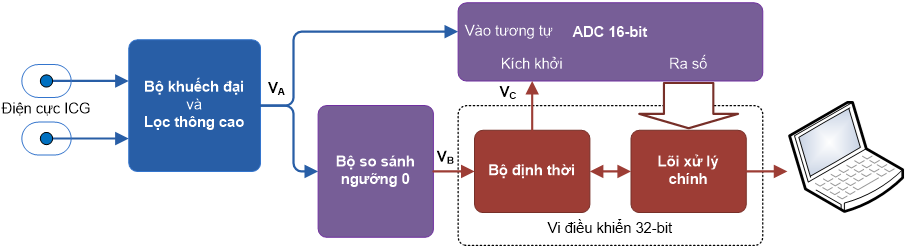
\includegraphics[width=16cm,height=4.39cm]{Images/hinh31.png}
    \caption[Sơ đồ khối của hệ thống]{\bfseries \fontsize{12pt}{0pt}\selectfont Sơ đồ khối của hệ thống}
    \label{hinh31}
\end{figure}
Hình \ref{hinh31} là ví dụ về cách chèn ảnh. Lưu ý chú thích của hình vẽ được đặt ngay dưới hình vẽ. Tất cả các hình vẽ phải được đề cập đến trong phần nội dung và phải được phân tích và bình luận giống như mình đang làm thế này nhé :)

\subsection{Cách tạo bảng}
\begin{table}[H]
    \centering
    \caption[Kết quả thí nghiệm]{\bfseries\fontsize{12pt}{0pt}\selectfont Kết quả thí nghiệm}
    \begin{tabularx}{0.85\textwidth}{
    | >{\centering\arraybackslash}y
    | >{\centering\arraybackslash}a
    | >{\centering\arraybackslash}a
    | >{\centering\arraybackslash}y|
    }
    \hline
    \bfseries  Lần thí nghiệm   &\bfseries Điện áp đo được \hspace{1cm}(mV)   &\bfseries Điện áp tham chiếu \hspace{0pt} (mV)  & \bfseries Sai lệch\hspace{0pt}(\%)\\\hline
       1  &   &   &\\\hline
       2  &   &   &\\\hline
       3  &   &   &\\\hline
    ...  &   &   &\\\hline
    \end{tabularx}
    \label{bang31}
\end{table}
Bảng \ref{bang31} là ví dụ về cách tạo bảng. Lưu ý chú thích của bảng được đặt ở trước bảng. Tất cả các bảng biểu phải được đề cập đến trong phần nội dung và phải được phân tích và bình luận giống như mình đang làm nhé :).

\begin{table}[ht]
\centering
\caption{A table without vertical lines.}
\begin{tabular}[t]{l|c|c}
\toprule
&Treatment A&Treatment B\\
\midrule
John Smith&1&2\\
\midrule
Jane Doe&--&3\\
\midrule
Mary Johnson&4&5\\
\bottomrule
\end{tabular}
\end{table}%

\subsection{Cách viết phương trình}
\begin{equation}\label{pt31}
    F(x) = \int^a_b \frac{1}{3}x^3
\end{equation}
Phương trình \ref{pt31} là ví dụ về phương trình tích phân. Từ phương trình \eqref{pt33} chúng ta tính được $y(t)$ như sau:
%
\begin{equation}\label{pt33}
    \int_{0}^{T}x(t)\times \delta t
\end{equation}

Thử phương trình khác nhé :)
\begin{equation}\label{pt32}
    x[t_n] = \frac{1}{\sqrt{N}} \sum_{k=0}^{N-1}X[f_k]e^{j 2\pi n k/N}
\end{equation}
Phương trình \ref{pt32} thể hiện phép biến đổi Fourier rời rạc ngược (IDFT).

\subsection{Cách viết định nghĩa, định lý, hệ quả, bổ đề,...}
Định lý lấy mẫu Nyquist-Shannon là một định lý được sử dụng trong lĩnh vực lý thuyết thông tin, đặc biệt là trong viễn thông và xử lý tín hiệu.
\begin{theorem}\label{đlNq} % Định lý
Một hàm số tín hiệu $x(t_n)$ không chứa bất kỳ thành phần tần số nào lớn hơn hoặc bằng một giá trị $f_m$ có thể biểu diễn chính xác bằng tập các giá trị của nó với chu kỳ lấy mẫu $T=1/(2f_m)$.
\end{theorem}
Định lý \ref{đlNq} thường được gọi đơn giản là định lý lấy mẫu.
\begin{corollary}\label{coro1}
this is something here about corollary.
\end{corollary}
Hệ quả \ref{coro1} gì đó ....
\begin{lemma}\label{lemma1}
đây là nội dung bổ đề.
\end{lemma}
Bổ đề \ref{lemma1} ....
\begin{defn}\label{defn1}
Nội dung định nghĩa...
\end{defn}
Định nghĩa \ref{defn1} nói về...
\newpage
\section*{CHƯƠNG 4. THÍ NGHIỆM VÀ KẾT QUẢ THÌ THẤY LÀ NẾU VIẾT HAI DÒNG SẼ BỊ XẤU}
\addcontentsline{toc}{section}{\numberline{}CHƯƠNG 4. THÍ NGHIỆM VÀ KẾT QUẢ}
\setcounter{section}{4}
\setcounter{figure}{0}
\setcounter{table}{0}
\lipsum
\begin{figure}[!ht]
    \centering
    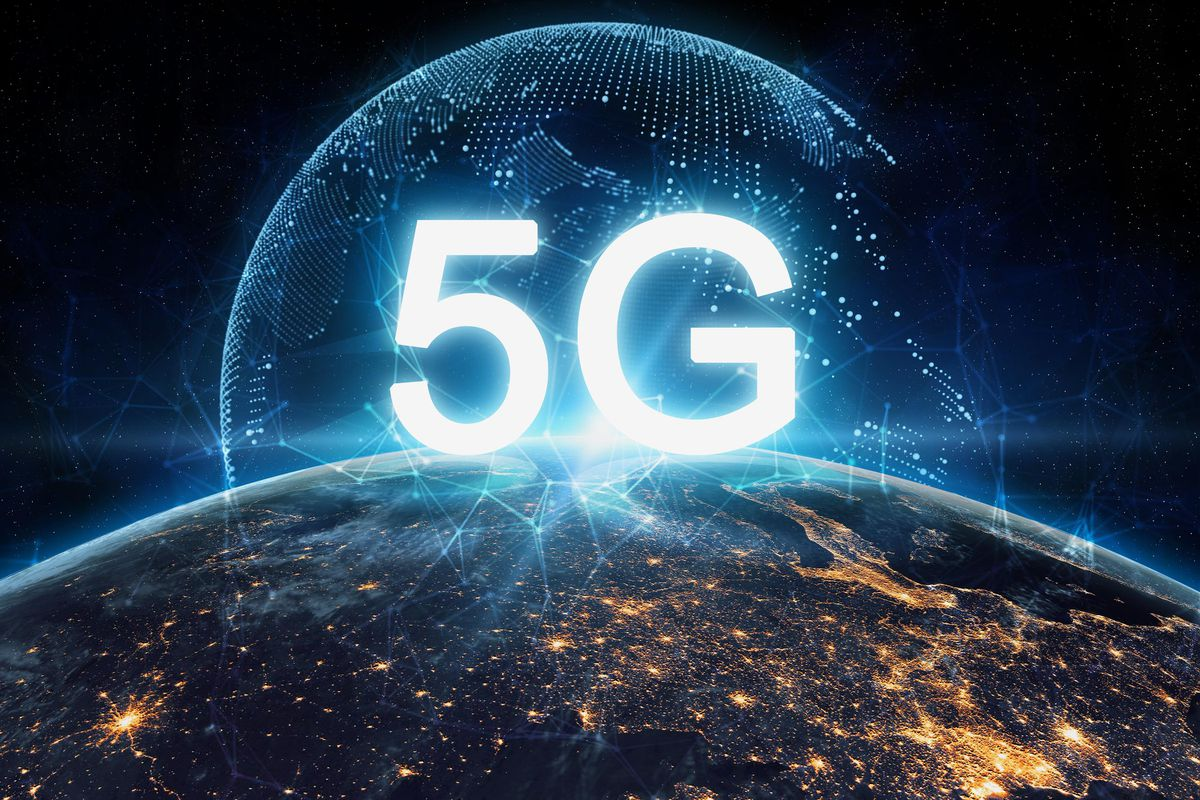
\includegraphics[width=16cm,height=6cm]{Images/5g.jpg}
    \caption[Mạng 5G]{\bfseries \fontsize{12pt}{0pt}\selectfont Mạng di động thế hệ thứ 5}
    \label{hinh41}
\end{figure}

Hình \ref{hinh41} là ví dụ về cách chèn ảnh. Lưu ý chú thích của hình vẽ được đặt ngay dưới hình vẽ. Tất cả các hình vẽ phải được đề cập đến trong phần nội dung và phải được phân tích và bình luận giống như mình đang làm thế này nhé :)
\newpage
\section*{KẾT LUẬN}
\phantomsection\addcontentsline{toc}{section}{\numberline {}KẾT LUẬN}
\subsection*{Kết luận chung}
\phantomsection\addcontentsline{toc}{section}{\numberline {}Kết luận chung}
Kết luận chung cho các chương trong đồ án. Mục này cần nhấn mạnh những vấn đề đã giải quyết và vấn đề chưa giải quyết để đưa ra các đánh giá về mức độ hoàn thành công việc. Đánh giá này thường bao gồm việc so sánh kết quả thu được với mục tiêu đề ra ban đầu.

Thêm một reference trước Li thì thế nào \cite{Yang2020}.

Ở đây chúng ta sẽ tập trích dẫn đến tài liệu tham khảo của Li \cite{Li2018}.

Bắt đầu với công thức toán số \eqref{congthuctinhtong} như sau:

\begin{equation}\label{congthuctinhtong}
    \sum_{i=1}^N x_i(t) = \Delta.
\end{equation}

\subsection*{Hướng phát triển}
\phantomsection\addcontentsline{toc}{section}{\numberline {}Hướng phát triển}
(Nếu có)
\subsection*{Kiến nghị và đề xuất}
\phantomsection\addcontentsline{toc}{section}{\numberline {}Kiến nghị và đề xuất}
(Nếu có)
\newpage
\phantomsection\addcontentsline{toc}{section}{\numberline {}TÀI LIỆU THAM KHẢO}
\bibliographystyle{IEEEtran}
\bibliography{MyRef}
\newpage
\section*{APPENDIX}
\phantomsection\addcontentsline{toc}{section}{\numberline{} APPENDIX}
\texttt{
\fontsize{10pt}{0pt}\selectfont Mã nguồn chương trình (nếu có) được đưa vào đây, sử dụng font Courier New, cỡ 10pt.} % Phụ lục nếu có
\end{document}

